\documentclass[a5paper,headsepline,titlepage,11pt,nnormalheadings]{scrbook}
\usepackage[a5paper,backref]{hyperref}
%\usepackage[papersize={148.5mm,215mm},twoside,bindingoffset=0.5cm,hmargin={2cm,2cm},
%				vmargin={2cm,2cm},footskip=1.1cm,driver=dvipdfm]{geometry}
\usepackage[papersize={107.5mm,148.5mm},twoside,bindingoffset=0.25cm,hmargin={1cm,1cm},
				vmargin={1.5cm,1.5cm},footskip=0.55cm,driver=dvipdfm]{geometry}
				
%\usepackage{palatino}
\usepackage{graphicx}
\usepackage{wrapfig}
\usepackage[bahasa]{babel}
\usepackage{fancyhdr}
\usepackage{longtable}
\usepackage{hhline,multirow}
\usepackage{pst-node}

%\setlength{\voffset}{0.5in}
%\setlength{\oddsidemargin}{28pt}
%\setlength{\evensidemargin}{0pt}
\renewcommand{\footrulewidth}{0.5pt}
\lhead[\fancyplain{}{\thepage}]%
      {\fancyplain{}{~}}
\rhead[\fancyplain{}{~}]%
      {\fancyplain{}{\thepage}}
\pagestyle{fancy}
\lfoot[\emph{Pesta Nama}]{}
\rfoot[]{\emph{Lingkungan St Petrus Maguwo}}
\cfoot{}

\newcommand{\BU}[1]{\begin{itemize} \item[U:] #1 \end{itemize}}
\newcommand{\BI}[1]{\begin{itemize} \item[I:] #1 \end{itemize}}
\newcommand{\BP}[1]{\begin{itemize} \item[P:] #1 \end{itemize}}
\newcommand{\BIP}[1]{\begin{itemize} \item[Bpk:] #1 \end{itemize}}
\newcommand{\BIW}[1]{\begin{itemize} \item[Ibu:] #1 \end{itemize}}
\newcommand{\namaromo}{~}
%lagu-lagu
\newcommand{\lagupembukaan}{~ }
\newcommand{\lagukyrie}{~ }
\newcommand{\lagugloria}{~}
\newcommand{\laguantarbacaan}{~ }
\newcommand{\lagubaitpengantarinjil}{~}
\newcommand{\lagupersembahan}{~ }
\newcommand{\lagusanctus}{~ }
\newcommand{\lagubapakami}{~ }
\newcommand{\laguagnusdei}{~}
\newcommand{\lagukomuni}{~}
\newcommand{\lagupenutup}{~ }

\hyphenation{sa-u-da-ra-ku}
\hyphenation{ke-ri-ngat}
\hyphenation{je-ri-tan}
\hyphenation{hu-bung-an}
\hyphenation{me-nya-dari}
\hyphenation{Eng-kau}
\hyphenation{ke-sa-lah-an}
\hyphenation{ba-gai-ma-na}
\hyphenation{Tu-han}
\hyphenation{di-per-ca-ya-kan}
\hyphenation{men-ja-uh-kan}
\hyphenation{bu-kan-lah}
\hyphenation{per-sa-tu-kan-lah}
\hyphenation{ma-khluk}
\hyphenation{Sem-buh-kan-lah}
\hyphenation{ja-lan}
\hyphenation{mem-bu-tuh-kan}
\hyphenation{be-ri-kan-lah}
\hyphenation{me-ra-sa-kan}
\hyphenation{te-man-ilah}
\hyphenation{mem-bi-ngung-kan}
\hyphenation{di-ka-gum-i}
\hyphenation{ta-ngis-an-Mu}
\hyphenation{mi-lik-ilah}


\renewcommand*\thesection{\arabic{section}.}

\makeatletter
\newcommand{\lagu}[1]{%
  {\parindent \z@ \normalfont
    \interlinepenalty\@M \bfseries \emph{#1}\par\nobreak \vskip 20\p@ }}
\setlength{\parindent}{0mm} 
\makeatother

\begin{document}
\thispagestyle{empty}
%\maketitle
%\newsavebox\IBox
%\sbox\IBox{\includegraphics[scale=0.4]{Saint-Peter-Apostle-e.eps}}

\psset{unit=1in}
\begin{pspicture}(4in,6.0in)
% set up the fonts we use
\DeclareFixedFont{\PT}{T1}{ppl}{b}{it}{0.4in}
\DeclareFixedFont{\PTsmall}{T1}{ppl}{b}{it}{0.3in}
\DeclareFixedFont{\PTsmallest}{T1}{ppl}{b}{it}{0.2in}
\DeclareFixedFont{\PTtext}{T1}{ppl}{b}{it}{11pt}
\DeclareFixedFont{\Logo}{T1}{pbk}{m}{n}{0.2in}
% place the front cover picture
%\rput[cb](2.3,2.5){\usebox\IBox}
% put the text on the front cover
\rput[cb](2.5,5.3){\PTsmall {Ekaristi Pesta Nama}}
\rput[cb](2.5,4.8){\PTsmall {Lingkungan St Petrus}}
\rput[cb](2.5,1.1){\PTsmall {29 Juni 2010}}
\rput[cb](2.5,0.6){\PTsmallest {Wilayah Yohanes de Britto}}
\rput[cb](2.5,0.3){\PTsmallest {Stasi Maguwo}}
\rput[cb](2.5,0.0){\PTsmallest {Paroki Marganingsih Kalasan }}

%\rput[cb](3,-1){\PTsmallest {\namagereja}} 

\end{pspicture}
%\tableofcontents 
\newpage
\thispagestyle{empty}
{~}
\newpage
\setlength{\parskip}{2mm}

\section*{RITUS PEMBUKA}
\lagu{Lagu pembuka \lagupembukaan}

\subsection*{SALAM PEMBUKAAN}
\BI{Atas nama Bapa Putera dan Roh Kudus} 
\BU{Amin}
\BI{Semoga damai sejahtera Tuhan kita Yesus Kristus, cinta kasih Allah Bapa dan persekutuan Roh Kudus, selalu beserta kita.}
\BU{Sekarang dan selama-lamanya}

\subsection*{PENGANTAR}
\BI{Bapak Ibu Saudara Saudari Anak-anak yang terkasih dalam Kristus, malam ini kita berkumpul untuk merayakan pesta nama Lingkungan Santo Petrus. Sebagai batu karang, Petrus merupakan landasan yang kokoh bagi kehidupan beriman kita. Kita berharap agar iman kita tetap tegar walaupun menghadapi cobaan yang berat di dunia ini.}

\emph{Hening sejenak \dots}
  
\subsection*{PERNYATAAN TOBAT}
\BI{Saudara-saudari yang seiman dalam Kristus, marilah kita membuat diri pantas berada di depan Allah, bersih dari dosa dan kesalahan yang lalu, dengan bertobat dan mohon ampun kepada Allah kita.}

\BI{Saya mengaku \dots}

\BI{Semoga Allah yang mahakuasa mengasihani kita, 
mengampuni dosa kita dan mengantar kita ke dalam hidup 
yang kekal.}

\BU{Amin}

\subsection*{Doa Pembuka} 
\BI{Marilah Berdoa 

Allah yang mahabaik, kami mengucap syukur kepada-Mu karena Engkau senantiasa mendengar dan memperhatikan kami dalam suka dan duka serta selalu menyertai kami dalam perjalanan hidup kami. Kami mohon, semoga iman kami kepadaMu tetap teguh sehingga dapat mengabdi kepadaMu dengan gembira dan penuh rasa syukur. Demi Yesus Kristus, PutraMu, Tuhan dan Pengantara kami, yang hidup dan berkuasa bersama Dikai dan Roh Kudus, kini dan sepanjang masa.
 }

\BU{Amin} 
 
\section*{IBADAT SABDA}
\BI{Saudara-saudari terkasih marilah kita mempersiapkan hati 
dan budi untuk mendengarkan sabda Tuhan.} 

\subsection*{BACAAN PERTAMA}

\BP{Pembacaan dari Kisah Para Rasul (12: 1-11) 

Kira-kira pada waktu itu raja Herodes mulai bertindak dengan keras terhadap beberapa orang dari jemaat.
Ia menyuruh membunuh Yakobus, saudara Yohanes, dengan pedang.
Ketika ia melihat, bahwa hal itu menyenangkan hati orang Yahudi, ia melanjutkan perbuatannya itu dan menyuruh menahan Petrus. Waktu itu hari raya Roti Tidak Beragi.
Setelah Petrus ditangkap, Herodes menyuruh memenjarakannya di bawah penjagaan empat regu, masing-masing terdiri dari empat prajurit. Maksudnya ialah, supaya sehabis Paskah ia menghadapkannya ke depan orang banyak.

Demikianlah Petrus ditahan di dalam penjara. Tetapi jemaat dengan tekun mendoakannya kepada Allah.
Pada malam sebelum Herodes hendak menghadapkannya kepada orang banyak, Petrus tidur di antara dua orang prajurit, terbelenggu dengan dua rantai. Selain itu prajurit-prajurit pengawal sedang berkawal di muka pintu.

Tiba-tiba berdirilah seorang malaikat Tuhan dekat Petrus dan cahaya bersinar dalam ruang itu. Malaikat itu menepuk Petrus untuk membangunkannya, katanya: "Bangunlah segera!" Maka gugurlah rantai itu dari tangan Petrus.
Lalu kata malaikat itu kepadanya: "Ikatlah pinggangmu dan kenakanlah sepatumu!" Iapun berbuat demikian. Lalu malaikat itu berkata kepadanya: "Kenakanlah jubahmu dan ikutlah aku!"
Lalu ia mengikuti malaikat itu ke luar dan ia tidak tahu, bahwa apa yang dilakukan malaikat itu sungguh-sungguh terjadi, sangkanya ia melihat suatu penglihatan.

Setelah mereka melalui tempat kawal pertama dan tempat kawal kedua, sampailah mereka ke pintu gerbang besi yang menuju ke kota. Pintu itu terbuka dengan sendirinya bagi mereka. Sesudah tiba di luar, mereka berjalan sampai ke ujung jalan, dan tiba-tiba malaikat itu meninggalkan dia.
Dan setelah sadar akan dirinya, Petrus berkata: "Sekarang tahulah aku benar-benar bahwa Tuhan telah menyuruh malaikat-Nya dan menyelamatkan aku dari tangan Herodes dan dari segala sesuatu yang diharapkan orang Yahudi."


Demikianlah sabda Tuhan }

\BU{Syukur kepada Allah} 

\lagu{Mazmur Tanggapan} 

\subsection*{BACAAN KEDUA}

\BP{Pembacaan dari Surat kedua Rasul Paulus kepada Timotius (4: 6-8,17-18) 

Saudara-saudara, mengenai diriku, darahku sudah mulai dicurahkan sebagai persembahan dan saat kematianku sudah dekat. Aku telah mengakhiri pertandingan yang baik, aku telah mencapai garis akhir dan aku telah memelihara iman.

Sekarang telah tersedia bagiku mahkota kebenaran yang akan dikaruniakan kepadaku oleh Tuhan, Hakim yang adil, pada hari-Nya; tetapi bukan hanya kepadaku, melainkan juga kepada semua orang yang merindukan kedatangan-Nya.

Tetapi Tuhan telah mendampingi aku dan menguatkan aku, supaya dengan perantaraanku Injil diberitakan dengan sepenuhnya dan semua orang bukan Yahudi mendengarkannya. Dengan demikian aku lepas dari mulut singa.
Dan Tuhan akan melepaskan aku dari setiap usaha yang jahat. Dia akan menyelamatkan aku, sehingga aku masuk ke dalam Kerajaan-Nya di sorga. Bagi-Nyalah kemuliaan selama-lamanya! Amin.

Demikianlah sabda Tuhan }

\BU{Syukur kepada Allah} 

\lagu{Bait pengantar Injil}

\subsection*{Bacaan Injil} 

\BI{Tuhan sertamu} 
\BU{Dan sertamu juga} 
\BI{Inilah Injil Yesus Kristus menurut Matius (16:13-19)} 
\BU{Dimuliakanlah Tuhan}

\BI{Setelah Yesus tiba di daerah Kaisarea Filipi, Ia bertanya kepada murid-murid-Nya: "Kata orang, siapakah Anak Manusia itu?"
Jawab mereka: "Ada yang mengatakan: Yohanes Pembaptis, ada juga yang mengatakan: Elia dan ada pula yang mengatakan: Yeremia atau salah seorang dari para nabi."
Lalu Yesus bertanya kepada mereka: "Tetapi apa katamu, siapakah Aku ini?"
Maka jawab Simon Petrus: "Engkau adalah Mesias, Anak Allah yang hidup!"
Kata Yesus kepadanya: "Berbahagialah engkau Simon bin Yunus sebab bukan manusia yang menyatakan itu kepadamu, melainkan Bapa-Ku yang di sorga.

Dan Akupun berkata kepadamu: Engkau adalah Petrus dan di atas batu karang ini Aku akan mendirikan jemaat-Ku dan alam maut tidak akan menguasainya.
Kepadamu akan Kuberikan kunci Kerajaan Sorga. Apa yang kauikat di dunia ini akan terikat di sorga dan apa yang kaulepaskan di dunia ini akan terlepas di sorga."

Demikianlah Injil Tuhan} 

\BU{Terpujilah Kristus}

\subsection*{HOMILI}

\subsection*{Syahadat (Aku Percaya)}

\subsection*{DOA UMAT}

\BI{Allah Bapa, melalui PutraMu, Yesus Kristus, Engkau mengundang kami datang kepadaMu agar kami memperoleh kelegaan, ketenangan dan keringanan atas beban hidup. Kami mohon, semoga Engkau mendengarkan doa-doa yang kami panjatkan ke hadiratMu:}

\BP{Bagi gereja:

Tuhan Allah kami, Engkau telah menghimpun kami dalam Gereja dan menguduskan kami menjadi umat pilihanMu. Semoga Gereja tetap berani dan tekun memberikan kesaksian tentang kehadiranMu di tengah dunia zaman ini.

Kami mohon}

\BU{Kabulkanlah doa kami ya Tuhan}

\BP{Bagi para Uskup, Imam, Diakon, dan pelayan Gereja lainnya:

Semoga para Uskup, Imam, Diakon, dan pelayan Gereja lainnya, selalu setia menghayati apa yang mereka wartakan dengan kesaksian hidup mereka.

Kami mohon}

\BU{Kabulkanlah doa kami ya Tuhan}

\BP{Bagi kita semua yang hadir di sini:

Allah, Bapa kami, kami bersyukur kepadaMu karena Yesus Kristus PutraMu telah berkenan menyatakan Engkau kepada kami. Semoga SabdaMu kuat berakar dan bertumbuh subur di dalam hati kami, serta mendorong kami untuk hidup damai dan saling mengampuni.

Kami mohon}

\BU{Kabulkanlah Doa kami ya Tuhan} 

\BP{Allah Bapa, berkatilah ikrar yang akan kami ucapkan agar menjadi pedoman kami dalam kehidupan menggereja dan bermasyarakat. Kuatkanlah hati dan tekad kami untuk teguh dalam melaksanakan ikrar tersebut.

Kami mohon}

\BU{Kabulkanlah doa kami ya Tuhan}

\BI{Demikianlah ya Bapa, doa-doa yang kami panjatkan. Engkau mengetahui keinginan keinginan dan kesulitan kami. Kami percaya akan penyelenggaraan-Mu dan bersama Roh Kudus. Kami menyampaikan doa-doa kami ini dengan perantaraan Putera-Mu terkasih, Tuhan kami Yesus Kristus, yang hidup dan berkuasa kini dan sepanjang masa. Amin}

\section*{LITURGI EKARISTI}

\subsection*{Persiapan Persembahan}

\lagu{Lagu persembahan: \lagupersembahan}

\subsection*{Doa Persembahan}

\BI{Allah Bapa kami yang Mahakudus, terimalah kiranya roti dan anggur yang kami persembahkan kepada-Mu ini. Satukanlah persembahan kami ini dengan kurban Yesus di altar ini. Sehingga persembahan kami menumbuhkan ketaatan dan memberikan kebahagian dan keselamatan bagi kami dan semua orang. Demi Kristus Tuhan dan pengantara kami.}

\BU{Amin}

\subsection*{Prefasi}

\lagu{Kudus: \lagusanctus}

\subsection*{Doa Syukur Agung}

\subsection*{Bapa Kami}
\lagu{\lagubapakami}

\subsection*{Salam Damai}

%\lagu{Anak Domba Allah: \laguagnusdei }

\subsection*{Persiapan Komuni}

\lagu{Lagu Komuni: \lagukomuni}

\section*{RITUS PENUTUP}

\subsection*{DOA PENUTUP}
\BI{Marilah berdoa :
 
Allah yang mahakuasa, kami bersyukur kepadaMu sebab melalui PutraMu, Engkau berkenan memanggil dan meringankan beban hidup kami serta mengajarkan kami untuk selalu hidup dalam kasih. Semoga iman kami semakin teguh mengakui segala kebaikanMu bagi kami. Demi Kristus, Pengantara kami. }
\BU{Amin} 

\subsection*{BERKAT}
\BI{Tuhan sertamu}
\BU{Dan sertamu juga}
\BI{Semoga kita semua yang hadir di sini senantiasa dibimbing dan dilindungi dengan limpahan berkat dari Allah Yang Maha Baik. ($\dagger$) Atas Nama Bapa, Putra, dan Roh Kudus}

\BU{Amin}

\BI{Saudara sekalian misa syukur kita sudah selesai marilah kita mundur dalam damai Tuhan}
\BU{Syukur kepada Allah.}

\lagu{Lagu penutup: \lagupenutup}

\end{document}